\documentclass[abstracton,12pt]{scrreprt}

\usepackage[utf8]{inputenc}
\usepackage[T1]{fontenc}
\usepackage{fancyhdr}
\usepackage{graphicx}
\usepackage{tikz}
\usepackage{times}
\usepackage{listings}
\usepackage{amssymb}
\usepackage{amsfonts}
\usepackage{amsmath}
\usepackage[
backend=bibtex,
style=alphabetic,
]{biblatex}

\addbibresource{bib.bib}


% --------- 

\titlehead{Department of Informatics, University of Zürich}
\subject{\vspace*{2cm}MSc Thesis}
\title{CAVIER}
\subtitle{Cascading View Trees}
\author{
  Johann Schwabe\\[-5pt]
  \scriptsize Matrikelnummer: 17-726-274\\[-5pt]
  \scriptsize Email: \texttt{johann.schwabe@uzh.ch}
}
\date{\vspace*{2cm}08.04.2023}
\publishers{
  \small supervised by Prof.\ Dr.\ D.\ Olteanu and Dr. H.\ Zhang \\[5cm]
  \begin{tikzpicture}[overlay]
    \node at (-3,-3) {
\includegraphics[height=1.5cm]{IFIlogo}};
    \node at (7,-3) {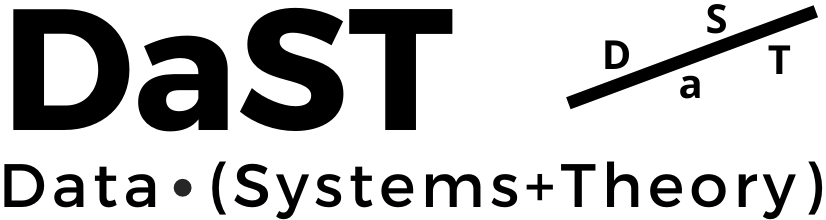
\includegraphics[height=1.5cm]{dast-logo}};
  \end{tikzpicture}
}

\dedication{dedicated to xxx}

% --------- 

\newtheorem{definition}{Definition}
\newtheorem{example}{Example}
\newtheorem{theorem}{Theorem}
\newtheorem{lemma}{Lemma}

\newenvironment{proof}
  {\noindent{\bf Proof:\rm}}{\hfill$\Box$\vspace{\medskipamount}}

\def\bbbr{{\rm I\!R}}
\def\bbbm{{\rm I\!M}}
\def\bbbn{{\rm I\!N}}
\def\bbbz{{\rm I\!Z}}

% --------- 

\begin{document}

\maketitle

\chapter*{Acknowledgements}

\begin{abstract}
  ...
\end{abstract}

\chapter*{Zusammenfassung}

\tableofcontents
\listoffigures
\listoftables

\chapter{Introduction}
Modern databases are under constant change (citetation needed). Thus their underlying database systems must efficiently handle these additions and deletions of tuple. But they must not only update the underlying data and their indices but also the views, presenting important information computed from the data to the users. As many traditional database systems cannot efficiently maintain these views, systems like FIVM were developped to improve on this. While FIVM can efficiently maintain individual views, every view is maintained individually without reusing shared subqueries between similar views. CAVIER, an extension of FIVM, presented in this thesis removes this limitation by focusing on maintaining a group of views and reusing results from previously computed views. Doing so, CAVIER can achieve asymtotically lower computation time than would be possible when individually maintaining the views using FIVM

\chapter{Foundations}
\section{Conjunctive Queries}
Conjunctive Queries are the key operation in any database system. They are joins over equality conditions. Conjunctive Queries also allow for  aggregations and grouping. Thus a Conjunctive Query consists of a set of base Relations $R_1, R_2, ..., R_i$ and join conditions between these relations. An example for a Join Condition is $R_j.1 = R_k.2$ describing that the first variable in Relation $R_j$ and the second attribute of $R_k$ have to be equal. Additionally the aggregation and grouping of variables is described by the free variables and semi-rings. Every Conjunctive Query defines a set of free variables by which the result is grouped by $R_j.l | (j,l) \in \textbf{Free}$. All other variables are so called bounden variables and are aggregated away. The method of aggregation is given by the used Semi-Ring.

A simple subgroup of Conjunctive Queries are those where all join conditions are natural joins. In these queries, each variable in a relation is assumed to have a name and join only with variables in different relations of the same name. Thus, relation can be defined as $R_i(a,b, ...)$ and a query as $Q_1(c,d,...) =R_i(a, b, ...), R_j(b, ...), ...$ where the explicit join condition would be $R_i.2 = R_j.1$ and the free variables are $c,d,...$. While these natural join Conjunctive Queries are a subset of all Conjunctive Queries, they are easier to describe and all notion described later can be extended to non natural join Conjunctive Queries and thus in the following example natural joins are assumed.

\section{Views and Database Updates}
While saving the data within small tables in normal form is efficient, the data often becomes difficulte to use. For humans to understand them or to interface other programs, the data needs to be reassembeld and maybe even preprocessed. These listings of joined tables are called views. 

These views must be updated on all database changes to reflect the new state of the data. The most simple view update is the complete recomputation of the view. But this is not efficient and in cases with large datasets or frequent updates no feasible. An alternative is to trace the influence of the change in for a delta-query and only update individual tuples in the correct relations. To accelerate this, a group of updates can be processed as a batch, reducing the number of delta-queries needed. While this allows for faster updates, the database is no longer real-time.

\section{Factorized Databases}
Factorized Databases are an alternative form of representing tuples in a relation. Traditional databases save a list of tuples for each relation and compute the join over them on demand, returning again lists of tuples. Contrary, Factorized Databases decompose the relations, for each query to a tree using laws of relational algebra. Using the law of distributivity of the Cartesian Product over unions much of the redundant information within the traditional listing representation can be removed. Thus they are a succient and lossless compression of the data for a given query. As the tuples aren't explicitly listed, they have be enumerated and the enumeration time is dependant of the variable order and thus the query. 
The example from \cite{FactorizedDB} (Figure \ref{fig:factorizedDBExample}) highlights the advantages well: While the listed result of the natural join of \textbf{Sales, Branch, Competition} uses 90 values, the factorized relation can compress the result to 20 values. Factorized databases aren't limited to joins but also support aggregation and group by clauses and can thus be used for most modern SQL queries.
The main drawback of factorized databases is that for each query a variable order needs to be found and for this variable order a Factorized representation built. Finding a good variable order is crucial to achieving a succient representation and thus efficient enumeration. \cite{FactorizedDB}
\begin{figure}
	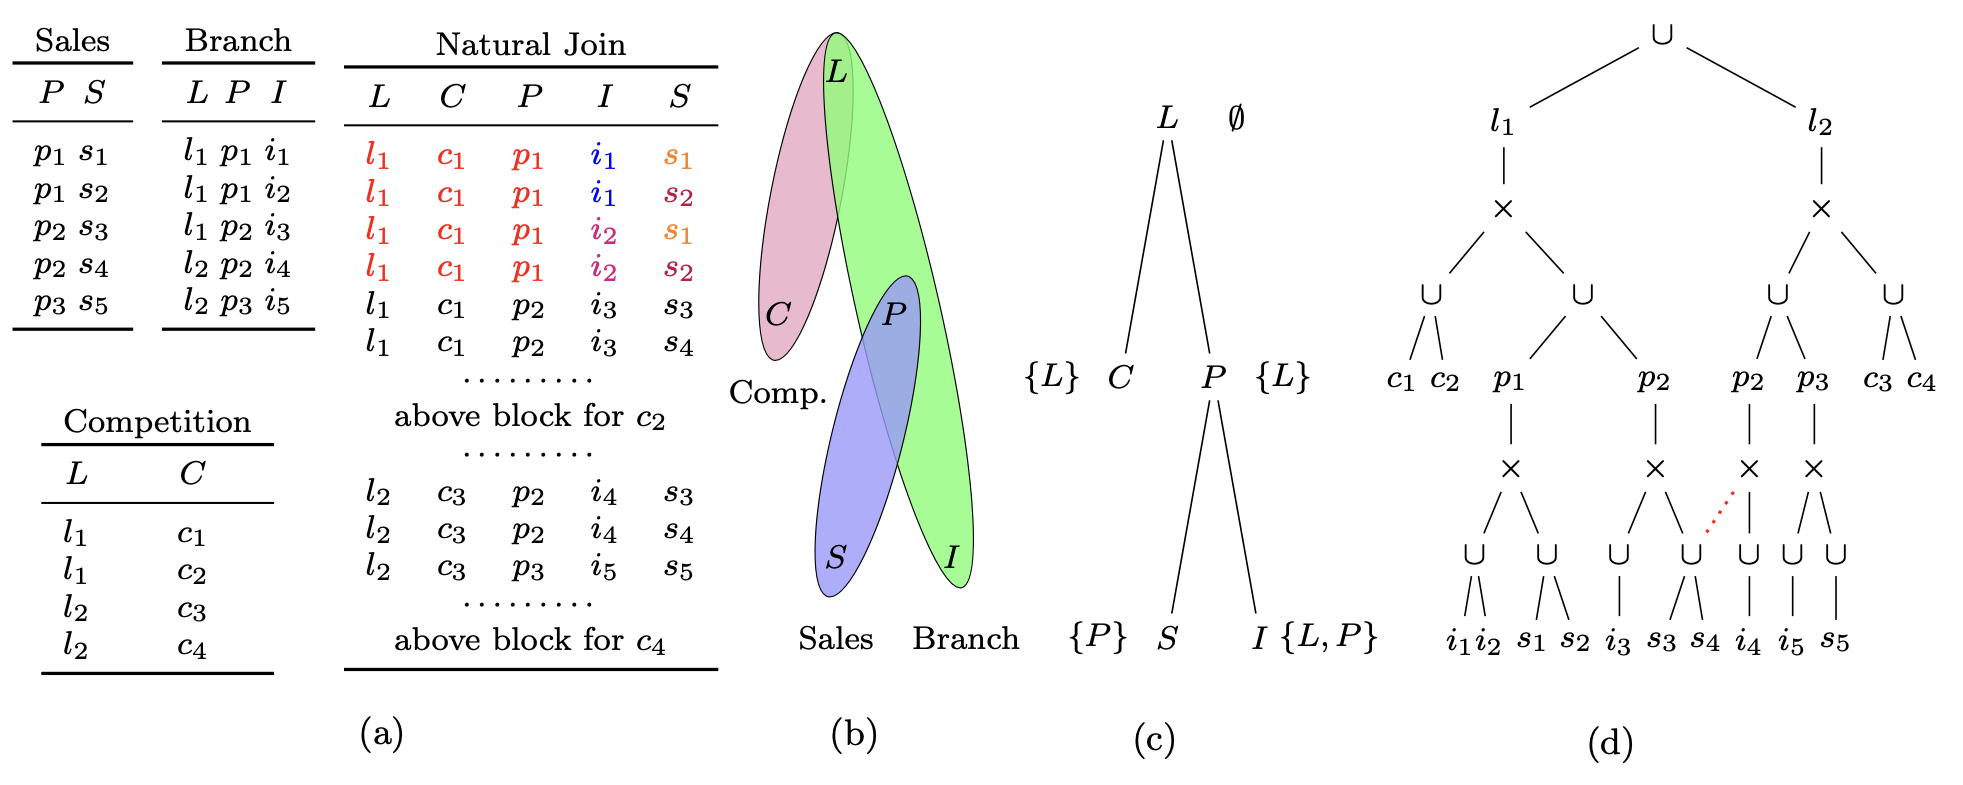
\includegraphics[width=\linewidth]{FactorizedExample.png}
	\caption{An example of a Factorized Database: a) Listing Representation, b) Hypergraph of the join, c) Variable order, d) Factorized Representation \cite{FactorizedDB}}
	\label{fig:factorizedDBExample}
\end{figure}


\subsection{Preprocesing vs enumeration vs update time}
The computational cost of a query can be split into three categories:
\begin{enumerate}
	\item  Preprocessing
	\item Enumeration
	\item Update
\end{enumerate}

\subsubsection{Preprocessing}
The preprocessing time is the time to build the support structure for the query when it is created. Thus it only occures once. If the database is assumed to be emty in the beginning, it is only the cost of building the support structures. If the query is created in a filled database, it also includes in filling the support structures with data. In this case, the preprocessing time can be at worst only the cost of creating the empty structure + the number of tuple times the update time.

\subsubsection{Enumeration}
The enumeration delay describes the maximum time it takes to list the next tuple based on the current state of the database. Thus the time to enumerate the whole output is the size of the output * the enumeration delay

\subsubsection{Update}
The update time is the maximum time needed to change the support structure on the addition or deletion of a tuple from any relation. After the update is completed the next tuples must enumerateable in the enumeration delay.

While the best database has a preprocessing time of O(1), and enumeration delay of O(1) and an update time of O(1), this is not possible for all database schemas and queries. For many databases a tradeof is needed. If there are few updates expected compared to enumeration requests, it is best to minimise the enumeration time, often at the cost of longer update times. (Citeation needed) optimal blabalablab

\subsection{Q-hierarchical}
Q-Hierarchical Queries are queries fullfilling the Q property and are Hierarchical. Q-Hierarchical queries are exactly those that allow for the optimal compute time of O(1) Preprocessing, O(1) Enumeration an O(1) Update time.

\subsubsection{Hierarichal}
By the definition from \cite{AnsweringConjunctiveQueriesUpdates}, a query is hierarchical iff for any two variables $ x, y \in vars(Q)$ it holds
$\text{atoms(}x\text{)} \subseteq \text{atoms(}y\text{) or atoms(}x\text{)} \supseteq \text{atoms(}y\text{) or atoms(}x\text{)} \cap \text{atoms(}y\text{) = }  \emptyset$

\subsubsection{Q}
By the same definition, a query is Q, iff for any two variables  $ x, y \in vars(Q)$ it holds:
$\text{if atoms(}x\text{)} \subsetneq \text{atoms(}y\text{) and } x \in \text{free(}Q\text{), then } y \in \text{free(}Q\text{)}$


\subsection{FIVM}
FIVM \cite{FIVM} is a database engine demonstrating the capabilities of Factorized Incremental View Maintainance. Given an SQL query it generates a view tree with its change rules for updates. This view tree is given in the intermediate file format M3 to a DB-Toaster \cite{dbtoaster} backend that builds a specialized database engine for this query and database schema. 
\subsection{DB-Toaster}

\chapter{Results}
\section{Cavier}
\subsection{Algorithm}
\subsection{Improvements}
\subsection{Limitations}
\subsection{Extensions}
\section{Benchmarks}

\chapter{Discussion}

\chapter{Conclusion}

\chapter{Appendix}

\printbibliography


\end{document}
